\section{Required Background}
\begin{frame}[fragile]{Required Background} 
\begin{block}{System Models}
\begin{enumerate}
  \item LTI drive model\pause
  \item LTI push model\pause
  \item Nonlinear push model
\end{enumerate}
\end{block}
\end{frame}

\begin{frame}[fragile]{Required Background} 
\begin{block}{Control Methods}
\begin{enumerate}
  \item Model Predictive Control (MPC)
  \item Model Predictive Path Intergral (MPPI) control
\end{enumerate}
\end{block}

% MPC and MPPI:
% Both have a objective function which they desire to miimize. 
% Robot wants to go go target, minimize distance to target. Now both methods caclulate the 
% input on the robot using two different methods. 

% MPC uses a system model to simulate the future states of the system whilst keeping robot input as variables to be determined
% Mathematical solvers then solve a minimization function that minimizes the objective function and find the robot input that 
% can be applied to the robot. The time step is incremented, new measurements are taken and a new minimization function is created 
% and the cycle repeats itself. Key thing to take away, robot input is found by mathematical solvers.

% MPPI simulate rollouts into the future. Using a system model and randomly generated input, multiple potential future states are
% obtained. The inputs that correspond to rollouts close to the desired states are mostly selected and inputs that correspond to
% rollouts far from the desired state are neglected. The multiple inputs are then combined into a single input, from which the 
% first input in applied to the system, the time step in incremented and the cycle repeats itself. 
\end{frame}


\begin{frame}[fragile]{Required Background} 
\begin{block}{Find a Path}
\begin{enumerate}
  \item Path Estimation\\
  \item Path Planning\\
\end{enumerate}
\end{block}
\end{frame}

\begin{frame}[fragile]{Required Background} 
  \todo{the robot inthe cente rplease}
  \begin{center}
  \hbox{\hspace{-0.5em} 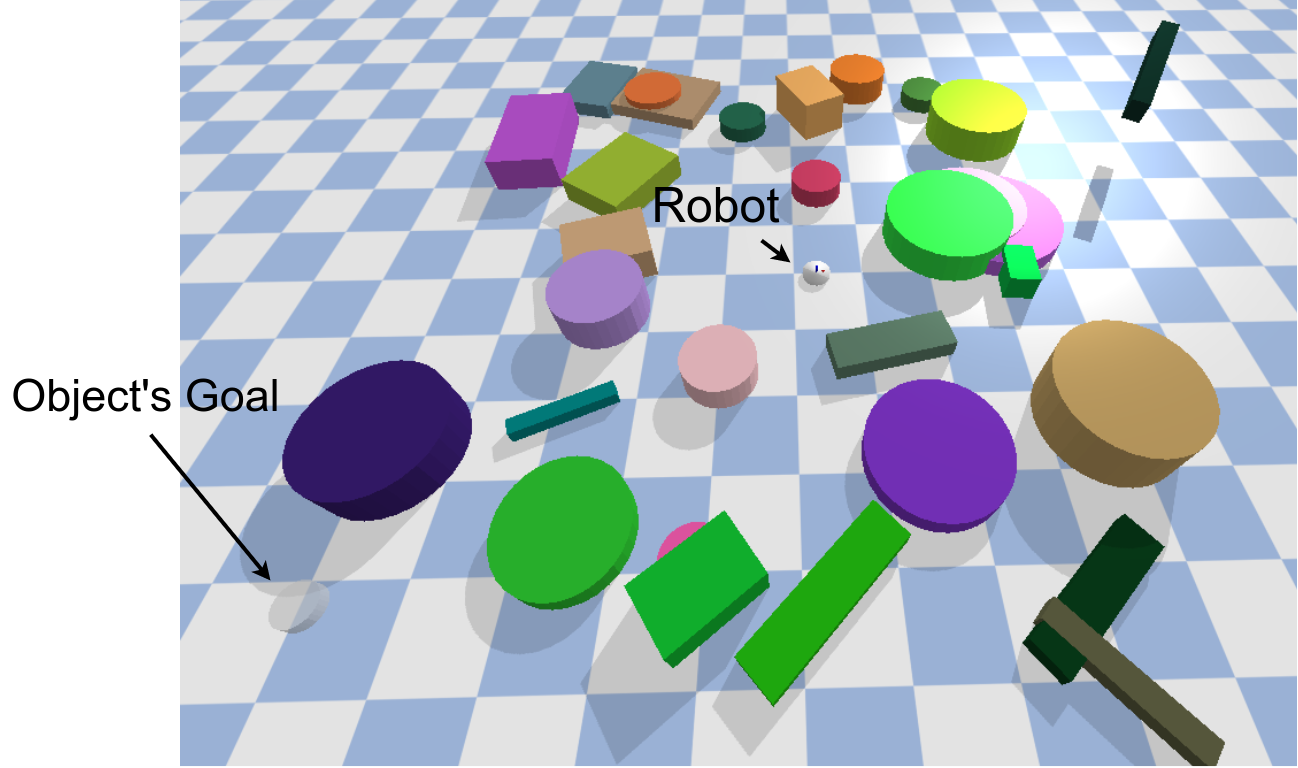
\includegraphics[width=1.0\textwidth]{figures/required_background/is_there_a_path}}
  \end{center}
\end{frame}

\begin{frame}[fragile]{Required Background} 
  \begin{center}
  \hbox{\hspace{-0.05\textwidth} 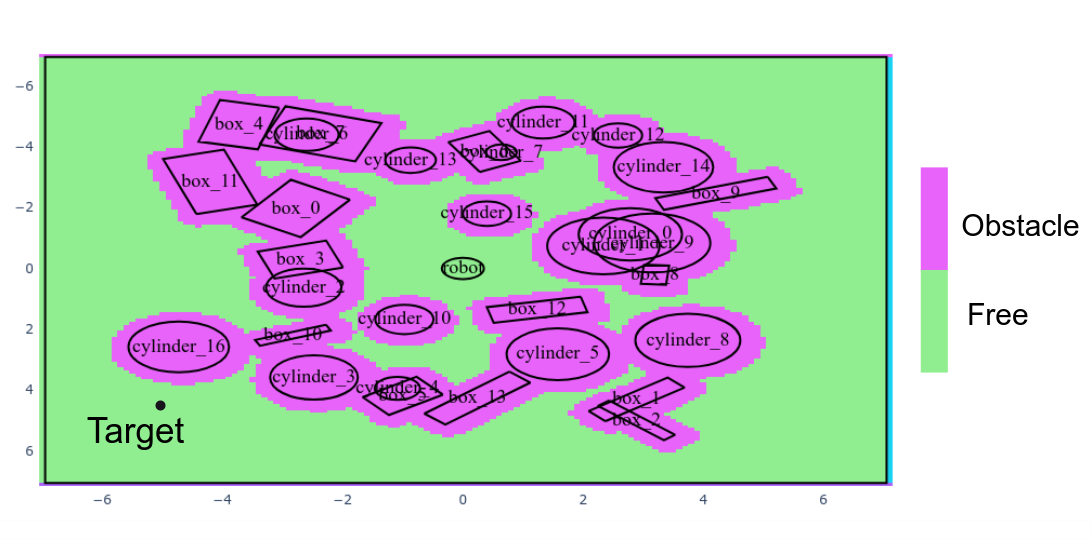
\includegraphics[width=1.1\textwidth]{figures/required_background/occupancy_grid} }
  \end{center}
\end{frame}

\begin{frame}[fragile]{Required Background} 

\begin{center}
\begin{tikzpicture}[scale=0.65, every node/.style={scale=0.65}]
    % Nodes
    \node [decision, text width=8em, line width=1pt] (first) {\huge Did Path estimator find a path? };

    \node [block, below left=1cm and 1cm of first, minimum width=13em, text width=16em, line width=1pt] (path_exists) {\huge Potentially Unfeasible };
    \node [block, below right=1cm and 1cm of first, minimum width=13em, text width=12em, line width=1pt] (path_does_not_exists) {\huge A path could still exist };

    \draw[>=stealth, ->, line width=1.0pt] (first.west) [out=180, in=90] to node[xshift=-0.3cm, above] {\huge yes} (path_exists.north);
    \draw[>=stealth, ->, line width=1.0pt] (first.east) [out=0, in=90] to node[xshift=0.3cm, above] {\huge no} (path_does_not_exists.north);
\end{tikzpicture}
\end{center}
\end{frame}

% \begin{frame}{GIFs in Beamer}
% \centering
% \animategraphics[loop,width=4cm]{10}{thanks-}{0}{6}
% \end{frame}


% \begin{frame}{GIFs in Beamer}
% \centering
% \movie[]{optional text}{figures/required_background/rrt.gif}
% \end{frame}


\begin{frame}[fragile]{Required Background} 
  \begin{center}
  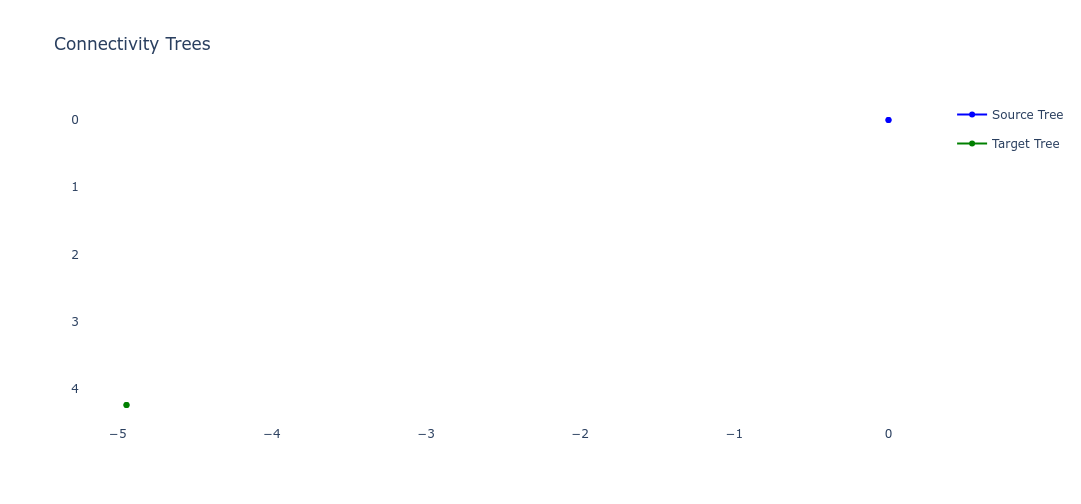
\includegraphics[width=1.0\textwidth]{figures/required_background/rrt/rrt0}
  \end{center}
\end{frame}

\begin{frame}[fragile]{Required Background} 
  \begin{center}
  \movie[width=\textwidth, height=0.5\textwidth, autostart, poster]{}{figures/required_background/rrtvideo.mp4}
  \end{center}
\end{frame}

\begin{frame}[fragile]{Required Background} 
  \begin{center}
  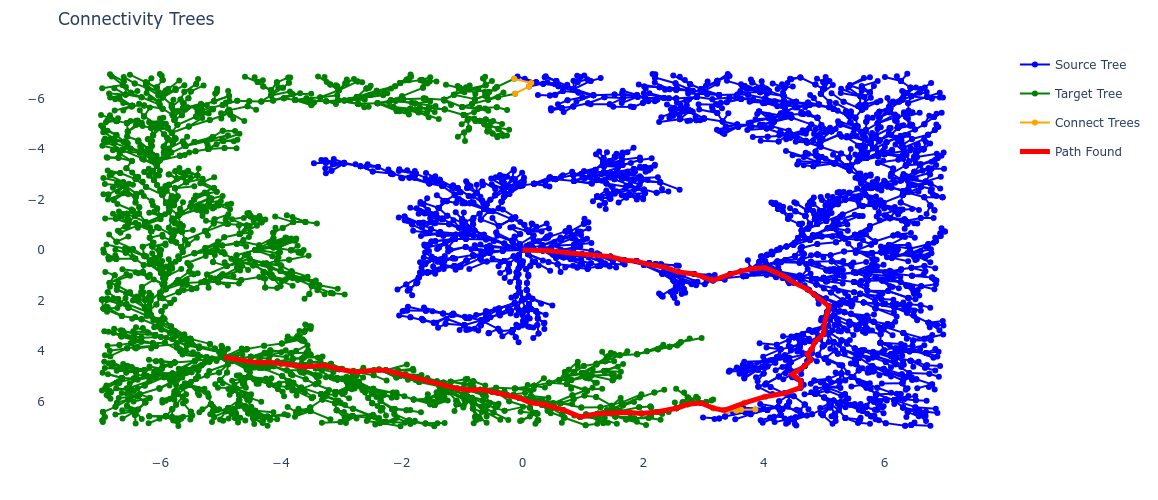
\includegraphics[width=1.0\textwidth]{figures/required_background/rrt/rrt67}
  \end{center}
\end{frame}

% \begin{frame}[fragile]{Required Background}
%   \centering
%   \animategraphics[width=\textwidth, autoplay, loop]{15}{figures/required_background/rrt/rrt}{0}{67}
% \end{frame}

% \animategraphics{fr}{figures/required_background/rrt.gif}{figures/required_background/rrtvideofirst}{figures/required_background/rrtvideolast}

% \begin{frame}[fragile]{Required Background} 

% \begin{center}
%     \includemedia[
%       width=0.6\linewidth,
%       height=0.4\linewidth,
%       activate=pageopen,
%       addresource=figures/required_background/rrtvideo.mp4,
%       flashvars={
%         source=figures/required_background/rrtvideo.mp4
%       }
%     ]{\fbox{Click to play}}{VPlayer.swf}
%   \end{center}
% \end{frame}

\begin{frame}[fragile]{Required Background} 
\[\mathit{Cost_{path}} = \sum_{i=1}^{n-1} \mathit{Distance}(c_i, c_{i+1})\]
\end{frame}


